\documentclass[a4paper,
			llpt,
			solution,
			accentcolor=tud2d,
			colorbacktitle
			]
			{tudexercise}

\usepackage[utf8]{inputenc}
%\usepackage[ngerman]{babel}
\usepackage{paralist}
\usepackage{amsmath}
\usepackage{pgfplots}
\pgfplotsset{compat=newest}
\usepgfplotslibrary{units}
%\usepgfplotslibrary{units}
\usepackage{xcolor}
%\definecolor{tud2d}{RGB}{0,78,115}
\definecolor{litegray}{gray}{0.5}

\usepackage{multicol} \setlength{\multicolsep}{0pt}

\title{Lösungsvorschlag zur vierten Hausübung}
\subtitle{Einführung in Net Centric Systems und \LaTeX, Sommersemester 2015}
\subsubtitle{Max Weller, Julian Haas, Stefan Pilot}

%\newcommand{\MiBs}{\frac{\mathrm{MiB}}{\mathrm{s}}}
\newcommand{\MiBs}{\mathrm{MiB}/\mathrm{s}}
\usepackage{multirow}
\newcommand{\8}{$\infty$}
\newcommand{\ezA}{\begin{tabular}{|c|c|c|c|c|c|}
\hline\multicolumn{2}{|c|}{\multirow{2}{*}{$\mathrm{D}^\mathrm{A}$}} & \multicolumn{4}{|c|}{Cost via}\\ \cline{3-6}\multicolumn{2}{|c|}{}& B & C & D & E\\ \hline\multirow{4}{*}{\rotatebox{90}{Destination}}}

\newcommand{\ezB}{\begin{tabular}{|c|c|c|c|c|c|}
\hline\multicolumn{2}{|c|}{\multirow{2}{*}{$\mathrm{D}^\mathrm{B}$}} & \multicolumn{4}{|c|}{Cost via}\\ \cline{3-6}\multicolumn{2}{|c|}{}& A & C & D & E\\ \hline\multirow{4}{*}{\rotatebox{90}{Destination}}}

\newcommand{\ezC}{\begin{tabular}{|c|c|c|c|c|c|}
\hline\multicolumn{2}{|c|}{\multirow{2}{*}{$\mathrm{D}^\mathrm{C}$}} & \multicolumn{4}{|c|}{Cost via}\\ \cline{3-6}\multicolumn{2}{|c|}{}& A & B & D & E\\ \hline\multirow{4}{*}{\rotatebox{90}{Destination}}}

\newcommand{\ezD}{\begin{tabular}{|c|c|c|c|c|c|}
\hline\multicolumn{2}{|c|}{\multirow{2}{*}{$\mathrm{D}^\mathrm{D}$}} & \multicolumn{4}{|c|}{Cost via}\\ \cline{3-6}\multicolumn{2}{|c|}{}& A & B & C & E\\ \hline\multirow{4}{*}{\rotatebox{90}{Destination}}}

\newcommand{\ezE}{\begin{tabular}{|c|c|c|c|c|c|}
\hline\multicolumn{2}{|c|}{\multirow{2}{*}{$\mathrm{D}^\mathrm{E}$}} & \multicolumn{4}{|c|}{Cost via}\\ \cline{3-6}\multicolumn{2}{|c|}{}& A & B & C & D\\ \hline\multirow{4}{*}{\rotatebox{90}{Destination}}}

\newcommand{\ze}{\end{tabular}}

\newcommand{\upd}{\begin{tabular}{c|c}}
\begin{document}
\maketitle
\section{Flooding}
\subsection{}
\begin{enumerate}
\item Siehe Grafik 1
\item Wie in Grafik 1 deutlich wird, führt der beschriebene Flooding Algorithmus angewendet auf die gegebene Topologie dazu, dass gewisse Pakete nie ankommen und in einer Schleife (Schritt 6 entspricht wieder Schritt 3) immer wieder hin und her geschickt werden. Selbst wenn eines der Pakete schon bei D angekommen ist und die Übertragung damit im Prinzip abgeschlossen ist, führt der Kreis in der Toplogie dazu, dass die Pakete immer weiter geschickt werden.
\item Der kürzeste Pfad von A nach D ist "ACBD". Da der kürzeste Pfad aus 3 "Sprüngen" besteht, wird mindestens ein hop count von 3 benötigt, damit die Pakete ankommen.
\end{enumerate}
\subsection{}
\begin{enumerate}

\item Siehe Grafik 2
\item Der hop count von 2 ist zu gering, um einen Pfad von A nach F zu finden. Deswegen werden die Pakete verworfen, bevor sie F erreichen können.
\item Der kürzeste Pfad von A nach F ist "ADEF". Der minimal benötigte hop count beträgt damit 3.
\item Keine, da der hop count hier 0 beträgt und die Router die Pakete deswegen nicht mehr weiter schicken dürfen.

\end{enumerate}
\subsection{}
\begin{enumerate}

\item siehe Tabelle.
%\begin{tabular}
%\\ \hline
%1 & 125\,ms    & 20\,$\MiBs$ & 10\,$\MiBs$ & 10\,$\MiBs$ \\ \hline
%2 & 208,33\,ms &  4\,$\MiBs$ & -6\,$\MiBs$ & 10\,$\MiBs$ \\ \hline
%3 & 166,67\,ms &  4\,$\MiBs$ &  0\,$\MiBs$ &  4\,$\MiBs$ \\ \hline
%4 & 500\,ms    &  0\,$\MiBs$ &  0\,$\MiBs$ &  0\,$\MiBs$ \\ \hline

%\begin{table}[ht]
%\caption{Die vier Phasen}
%\centering
%\begin{tabular}{|c|c|c|c|c|c|c|c|c|c|c|c|c|c|c|c|}
%\\ \hline
%Node & A & B & C & D & E & F & G & Sum \\ \hline
%Step & s & d & s  & d & s & d & s & d & s & d & s & d & s & d & Sum \\ \hline
%\end{tabular}
%\end{table}

\item KEINE AHNUNG???

\end{enumerate}
\subsection{}
      1. Jede Station merkt sich, welche Pakete sie schon gesendet hat und sendet diese kein zweites Mal. So lassen sich Dopplungen vermeiden.\\
      2. Selective Flooding: Die Stationen merken sich, aus welcher "Richtung" die Pakete kamen und versuchen die Pakete nur in "Zielrichtung" weiterzuschicken. Dies funktioniert zwar abhängig von der Netzwerktopologie nur sehr begrenzt, verhindert aber, dass Pakete z.B. wieder beim Absender landen.
\section{Autonomous Systems}
\section{Border Gateway Protocol}
\subsection{}
\begin{enumerate}
\item Provider Q kann bis zu drei Routen zu Provider P empfangen, nämlich über 1, über 2, und über 4-3.
\item Die Aufgabenstellung ist unklar, ich interpretiere es wie folgt: Traffic wird immer über die nächstgelegene Line geleitet, die zum Zielprovider führt. Das ist nennt sich auch Hot-Potato-Prinzip: Paket möglichst schnell aus dem eigenen Verantwortungsbereich herausrouten.

\begin{multicols}{2}
Dann fließt ein Paket von A zu B wie folgt:

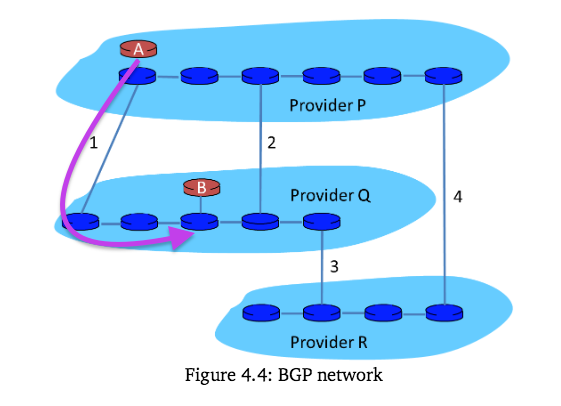
\includegraphics[scale=0.4]{4_3_1_b_AB.png}

Ein Paket von B zu A verläuft wie folgt:

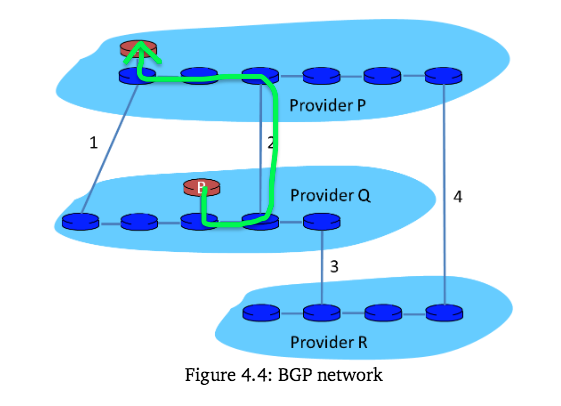
\includegraphics[scale=0.4]{4_3_1_b_BA.png}
\end{multicols}
\end{enumerate}
\subsection{}
\begin{multicols}{2}
Wie die Router in diesem Fall reagieren, kommt auf die Konfiguration an: Die Router sind vermutlich so konfiguriert, dass sie keine Routen aus BGP übernehmen, in deren AS-PATH sie selbst vorkommen. Dann wird der grün markierte Pfad verwendet. Es könnte aber auch von den Admins von AS42 explizit eingestellt sein, dass die Abkürzung über AS23 verwendet wird. \vfill \columnbreak
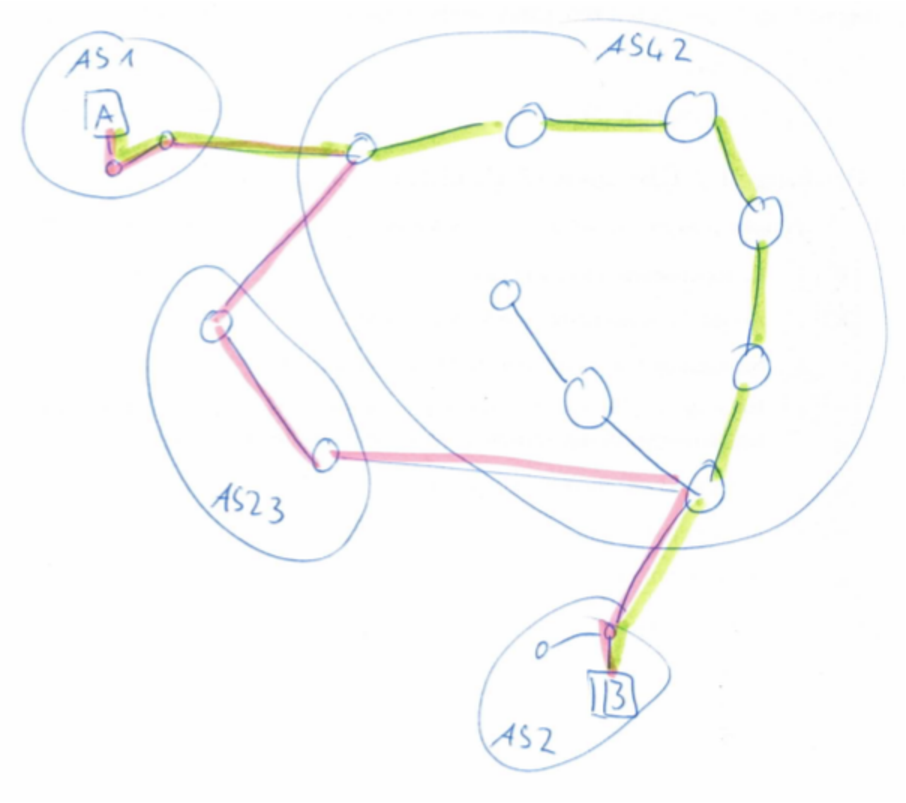
\includegraphics[scale=0.5]{4_3_2.pdf}
\end{multicols}
\subsection{}
BGP löst das Count-To-Infinity-Problem durch die Übertragung des kompletten bevorzugten Pfades (AS-PATH).
\\
Beispiel:
\begin{multicols}{2}
Ausgangssituation:
\begin{center}
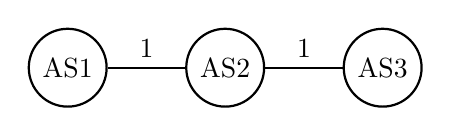
\begin{tikzpicture}[-,
					%>=stealth',
					%shorten >=1pt,
					auto,
					node distance=2cm,
					thick,
					main node/.style={circle,draw}]

  \node[main node] (A) {AS1};
  \node[main node] (B) [right of=A] {AS2};
  \node[main node] (C) [right of=B] {AS3};

  \path[every node/.style={}]
    (A) edge node {1} (B)
    (B) edge node {1} (C);
\end{tikzpicture}
\begin{tabular}{c|c|c|c}
von &  zu  &  AS-PATH &  Kosten \\ \hline
AS2 &  AS1 &   -      &   1 \\
AS3 &  AS1 &   AS2    &   2 \\
\end{tabular}
\end{center}
Der Link zwischen AS1 und AS2 wird schlechter:
\begin{center}
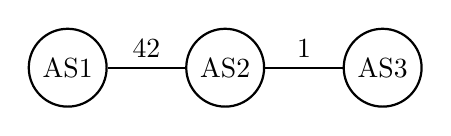
\begin{tikzpicture}[-,
					%>=stealth',
					%shorten >=1pt,
					auto,
					node distance=2cm,
					thick,
					main node/.style={circle,draw}]

  \node[main node] (A) {AS1};
  \node[main node] (B) [right of=A] {AS2};
  \node[main node] (C) [right of=B] {AS3};

  \path[every node/.style={}]
    (A) edge node {42} (B)
    (B) edge node {1} (C);
\end{tikzpicture}
\end{center}
AS2 bemerkt Abbruch des Links zu AS1, also:
\begin{center}
\begin{tabular}{c|c|c|c}
von &  zu &   AS-PATH &  Kosten \\ \hline
AS2 &  AS1 &   -    &    1 \\
\end{tabular}
\end{center}
wird gelöscht.\\
~\\
Gleichzeitig erhält AS2 aber folgende Route von AS3:
\begin{center}
\begin{tabular}{c|c|c|c}
von &  zu  &  AS-PATH &  Kosten \\ \hline
AS2 &  AS1 &  AS3,AS2  &  3 \\
\end{tabular}
\end{center}
Diese wird aber von AS2 verworfen, da im AS-PATH AS2 selber vorkommt. Damit wurde das Count-To-Infinity verhindert.
\end{multicols}

\subsection{}
Die Angreifer haben das BGP verwendet, um Internettraffic vom Nutzer unbemerkt über ihre eigenen Netze umzuleiten. Dazu wurde von einem Provider auf einem Uplink ein fremdes Prefix announced, sodass der Traffic in das Netz gelangt. Eine andere Route wurde unverändert gelassen, um den Traffic danach an das eigentliche Ziel weiterleiten zu können. Der Angreifer kann den Traffic dadurch abhören oder als MitM auch verändern.
\subsection{}
BGP ist ein auf path vector routing basierendes Routingprotokoll, welches für das Routing zwischen den Autonomen Systemen eingesetzt wird, aus denen das Internet besteht. Es wird daher auch als Exterior Gateway Protocol bezeichnet. \\
\begin{multicols}{2}
Vorteile: \begin{compactenum}
\item sehr flexibel da nur Distanz übertragen wird und Policyentscheidungen lokal vom Admin getroffen werden können
\item vermeidet Count-To-Infinity
\end{compactenum}
~\\
\vfill
\columnbreak
Probleme: \begin{compactenum}
\item Skalierung: Anzahl der AS steigt, die in jedem Router gespeicherte Tabelle aller erreichbaren Prefixe wird immer größer
\item Sicherheit: BGP ist anfällig für Spoofing, da normalerweise jeder Provider jedes Präfix announcen  kann
\end{compactenum}
\end{multicols}
\section{RIP and OSPF}
\subsection{Name at least 4 main characteristics of RIP.\\Briefly explain how the algorithm works.\\ What happens if a link goes down?}
Das Routing-Information-Protocol implementiert Distance-Vector-Routing. Dabei wird der Hop Count als Metrik eingesetzt. Die maximale Anzahl Hops liegt bei 15, 16 Hops sind gleichbedeutend mit \8, weshalb die maximale Netzwerkgröße begrenzt ist. RIP unterliegt dem Count-to-Infinity-Problem.\\
Alle 30 Sekunden senden alle Router in den sog. Response Messages ihre Routingtabelle an die direkt verbundenen Nachbarn, die dadurch ihre eigenen Routingtabelle aktualisieren können.\\
Empfängt ein Router 180 Sekunden lang keine Nachrichten, die darüber Aufschluss geben, dass ein ihm bekannter Router noch erreichbar ist, setzt er den Hop Count zu diesem Router auf 16 $\hat{=}$ \8.\\
Die genannten Zeitdauern sind die in RFC 1058 definierten Standardzeiten und können in manchen Implementierungen abweichen.
\subsection{How does the algorithm OSPF work?\\Additionally describe at least 2 main characteristics  of the protocol OSPF.\\Which additional features have been introduced in OSPF? Name at least 3 features.\\Briefly compare OSPF to RIP.}
Open Shortest Path First implementiert Link-State-Routing und benutzt Dijkstras "Shortest Path First"-Algorithmus. Nachdem alle Knoten das Gewicht der adjazenten Kanten herausgefunden haben, verschicken sie ein Paket mit diesen Informationen, welches per Flooding im Netzwerk verteilt wird. So kann sich jeder Router einen Graphen zeichnen, der das komplette Netzwerk repräsentiert und per Dijkstra den minimalen Spannbaum berechnen, nach welchem er dann routet.\\
OSPF weist gegenüber RIP zahlreiche neue Funktionen auf, unter anderem werden die Routingpakete per TCP verschickt und authentifiziert, OSPF unterstützt multiple Metriken für die gleiche Verbindung, Hierarchie und Subnetze durch die Einteilung des Netzwerks in Areas, VLSM, CIDR und routet garantiert loop-frei. OSPF unterliegt nicht dem Count-to-Infinity-Problem.\\
Im Vergleich zu RIP ist OSPF besser skalierbar und bietet geringere Konvergenzzeiten. Durch die geringere Anzahl nötiger Update Messages verursacht OSPF einen geringeren Overhead in großen Netzwerken. Da die Implemtierung allerdings sehr kompliziert ist und die einzelnen Knoten eine größere Rechenleistung brauchen als bei RIP ist OSPF für kleine Netzwerke nicht empfehlenswert.
\section{Overlay Routing}
\section{Multiple Choice}
\subsection{Which is the lowest layer that uses traffic regulation mechanisms to keep a fast transmitter from drowning a slow receiver in data?}
\begin{compactenum}
\item[d)] Data Link Layer
\end{compactenum}
\subsection{Which layer is responsible for determining how packets are routed from source to destination?}
\begin{compactenum}
\item[b)] Network Layer
\end{compactenum}
\subsection{Which kind of routing algorithms are variable according to the current network status?}
Das kommt darauf an, wie man "Status" definiert. Dynamische Routingalgorithmen sind in der Lage, den Ausfall von Knoten oder Verbindungen zu kompensieren. Adaptive Routingalgorithmen berücksichtigen auch die Auslastung einzelner Knoten und Verbindungen. Der Übergang ist allerdings fließend und hängt auch von der Metrik ab.
\begin{compactenum}
\item[a)] Adaptive routing algorithms
\item[d)] Dynamic routing algorithms
\end{compactenum}
\subsection{For which algorithms the count-to-infinity problem does not occur?}
\begin{compactenum}
\item[a)] LSR
\item[c)] BGP
\item[d)] OSPF
\item[f)] DSR
\end{compactenum}
\subsection{When a connection is established, a route from the source machine to the destination machine is chosen as a part of the connection setup and stored in tables inside the routers. For which connection is the statement valid?}
\begin{compactenum}
\item[b)]{Connection-oriented Services}
\end{compactenum}
\subsection{Which of the algorithms throws away tokens when a bucket fills up but never discards packets?}
\begin{compactenum}
\item Token Bucket
\end{compactenum}
\subsection{Which of the fields belong only to IPv6?}
\begin{compactenum}
\item[c)] Next header
\item[d)] Payload length
\item[f)] Hop limit
\end{compactenum}
\subsection{How do you call a connection that allows traffic either way but only one way at a time?}
\begin{compactenum}
\item[c)]{half duplex}
\end{compactenum}
\subsection{According to DVR all update messages are sent...}
\begin{compactenum}
\item[c)]{only to neighbouring nodes}
\end{compactenum}
\end{document}
